\documentclass[12pt]{article}
\setlength{\oddsidemargin}{0in}
\setlength{\evensidemargin}{0in}
\setlength{\textwidth}{6.5in}
\setlength{\parindent}{0in}
\setlength{\parskip}{\baselineskip}
\usepackage{amsmath,amsfonts,amssymb}
\usepackage{graphicx}
\usepackage[]{algorithmicx}
\usepackage{enumitem}
\usepackage{fancyvrb}
\usepackage{ wasysym }
\usepackage{tkz-berge}
\usetikzlibrary{positioning, automata}


\usepackage{fancyhdr}
\pagestyle{fancy}
\setlength{\headsep}{36pt}

\usepackage{hyperref}


\hypersetup{
    colorlinks=true,
    linkcolor=blue,
    filecolor=magenta,      
    urlcolor=blue,
}

\newcommand{\makenonemptybox}[2]{%
%\par\nobreak\vspace{\ht\strutbox}\noindent
\item[]
\fbox{% added -2\fboxrule to specified width to avoid overfull hboxes
% and removed the -2\fboxsep from height specification (image not updated)
% because in MWE 2cm is should be height of contents excluding sep and frame
\parbox[c][#1][t]{\dimexpr\linewidth-2\fboxsep-2\fboxrule}{
  \hrule width \hsize height 0pt
  #2
 }%
}%
\par\vspace{\ht\strutbox}
}
\makeatother

\begin{document}
\lhead{{\bf CSCI 3104, Algorithms \\ Homework 6 (100 points)} }
\rhead{Name: \fbox{% Place your name here and delete the next time
\phantom{This is a really long name}} 
\\ ID: \fbox{ % Place your ID here and delete the next time
\phantom{This is a student ID}} 
\\ {\bf Escobedo \& Jahagirdar\\ Summer 2020, CU-Boulder}}
\renewcommand{\headrulewidth}{0.5pt}

\phantom{Test}

\begin{small}
\textit{Advice 1}:\ For every problem in this class, you must justify your answer:\ show how you arrived at it and why it is correct. If there are assumptions you need to make along the way, state those clearly.
%\vspace{-3mm} 

\textit{Advice 2}:\ Verbal reasoning is typically insufficient for full credit. Instead, write a logical argument, in the style of a mathematical proof.\\
%\vspace{-3mm} 

\textbf{Instructions for submitting your solution}:
\vspace{-5mm} 

\begin{itemize}
	\item The solutions \textbf{should be typed}, we cannot accept hand-written solutions. Here's a short intro to \href{http://ece.uprm.edu/~caceros/latex/introduction.pdf}{\textbf{Latex}.}
	 \item In this homework we denote the asymptomatic \textit{Big-O} notation by $\mathcal{O}$ and \textit{Small-O} notation is represented as $o$. 
	\item We recommend using online Latex editor \href{https://www.overleaf.com/}{\textbf{Overleaf}}. Download the \textbf{.tex} file from Canvas and upload it on overleaf to edit.
	%todo add link of gradescope
	\item You should submit your work through \href{https://www.gradescope.com}{\textbf{Gradescope}}  only.
	\item If you don't have an account on it, sign up for one using your CU email. You should have gotten an email to sign up. If your name based CU email doesn't work, try the identikey@colorado.edu version. 
	\item Gradescope will only accept \textbf{.pdf} files (except for code files that should be submitted separately on Canvas if a problem set has them) and \textbf{try to fit your work in the box provided}. 
	\item You cannot submit a pdf which has less pages than what we provided you as Gradescope won't allow it.
   
\end{itemize}
\vspace{-4mm} 
\end{small}

\hrulefill
\pagebreak

\subsection*{Piazza threads for hints and further discussion}
\begin{center}
    \begin{tabular}{|c|}
    \hline
    Piazza Threads \\ [0.5ex] 
    \hline \hline 
    \href{https://piazza.com/class/ka2roz7rb9m3j4?cid=87}{Question 1}\\
    \href{https://piazza.com/class/ka2roz7rb9m3j4?cid=88}{Question 2}\\
    \href{https://piazza.com/class/ka2roz7rb9m3j4?cid=89}{Question 3}\\
    \href{https://piazza.com/class/ka2roz7rb9m3j4?cid=90}{Question 4}\\
    \href{https://piazza.com/class/ka2roz7rb9m3j4?cid=91}{Question 5}\\
    \href{https://piazza.com/class/ka2roz7rb9m3j4?cid=92}{Question 6}\\
    \href{https://piazza.com/class/ka2roz7rb9m3j4?cid=93}{Question 7}\\
    \href{https://piazza.com/class/ka2roz7rb9m3j4?cid=94}{Question 8}\\
    \hline
    \end{tabular}
\end{center}

\textbf{Recommended reading}: \\
Graph Algorithms Intro: Ch. 22 $\to$ 22.1, 22.2, 22.3 \\
Graph Algorithms SSSPs: Ch. 24 $\to$ 24.3
\\

\pagebreak

\begin{enumerate}
    
     \item (5 pts) How many unique MSTs does the following graph have. Show the necessary work to justify your answer. 
    \begin{figure}[h!]
    \begin{center}
    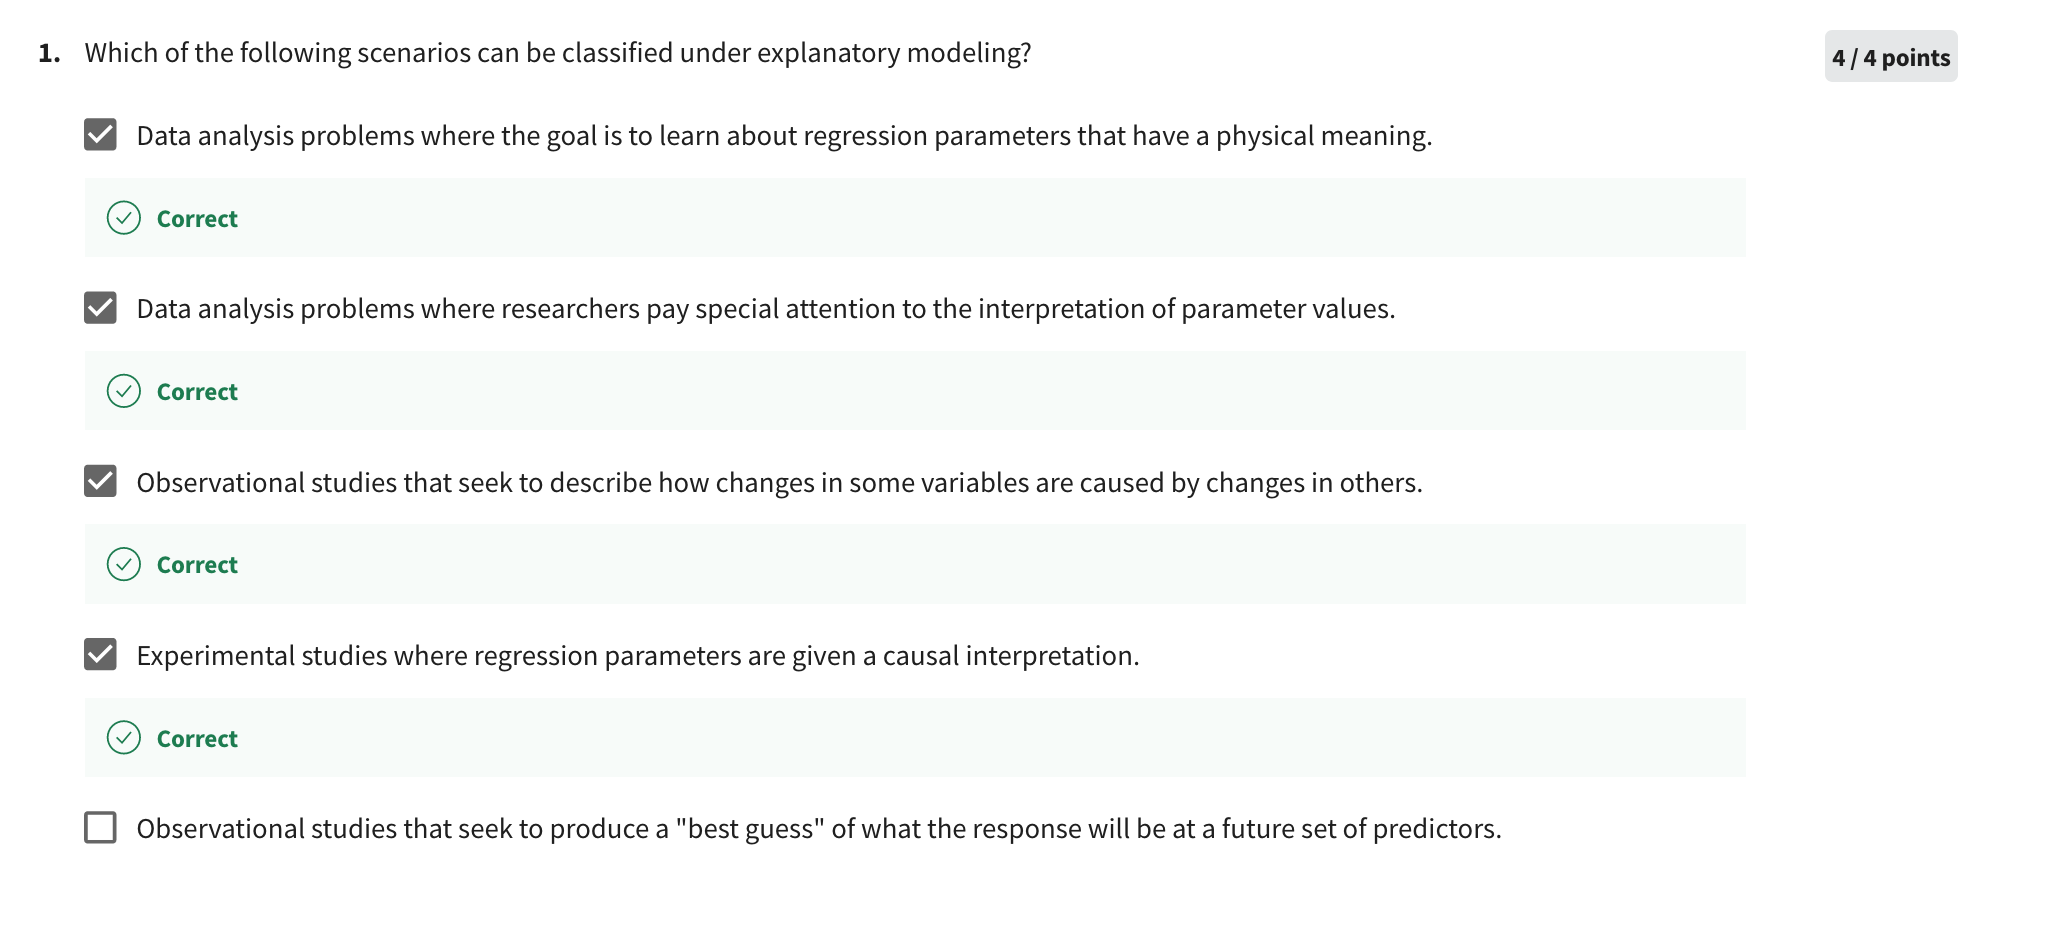
\includegraphics[scale=1]{HW6/p1.PNG} 
    \end{center}
    \end{figure}
    \makenonemptybox{4in}{}

    \item (20 pts) Based on the following graph :
    \begin{figure}[h!]
    \begin{center}
    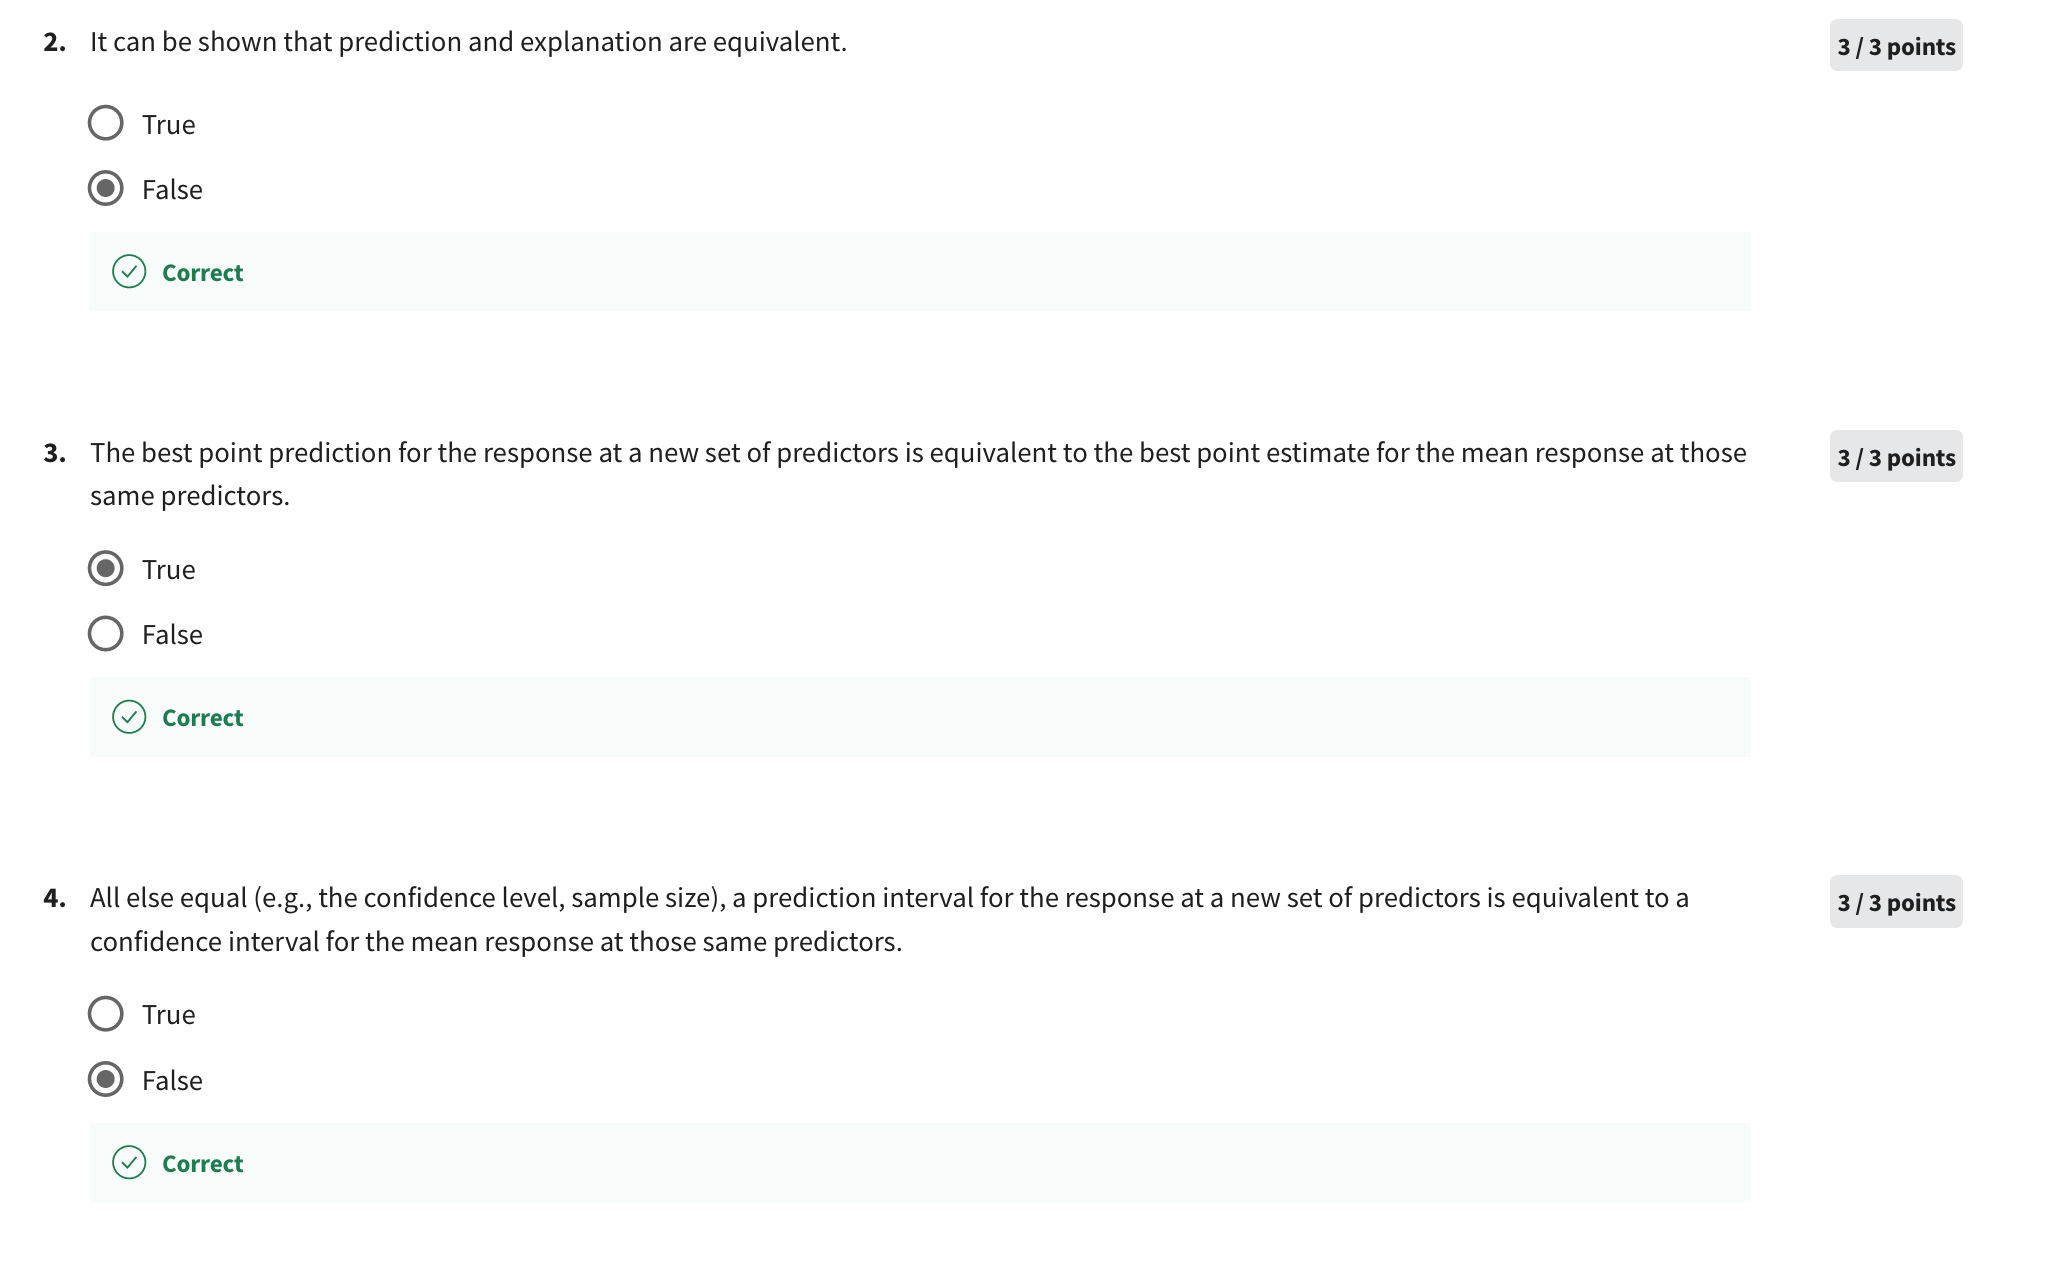
\includegraphics[scale=1]{HW6/p2.png} 
    \end{center}
    \end{figure}

    \begin{enumerate}[label=(\alph*)]
        \item (10 pts) In what order would Prim's algorithm add edges to the MST if we start at     vertex $A$? 
        \makenonemptybox{3in}{}
        \clearpage
        \item (10 pts) In what order Kruskal's would add the edges to the MST? 
        \makenonemptybox{6in}{}
    \end{enumerate}
    \clearpage
    
    \item (10 pts) Suppose that you have calculated the MST of an undirected graph $G=(V,E)$ with positive edge weights.  If you increase each edge weight by 5, will the MST change? Prove that it cannot change or give a counterexample if it changes. (Note: Your proof, if there is one, can be a simple logical argument.)
  
    \makenonemptybox{6in}{}
	\clearpage

    \item (15 pts) Suppose you are given the minimum spanning tree $T$ of a given graph G (with $n$ vertices and $m$ edges) and a new edge $e=(u,v)$ of weight $w$ that will be added to $G$. Give an efficient algorithm to find the MST of the graph $G\cup e$. Your algorithm should run in $O(n)$ time.\\
	\makenonemptybox{6in}{}
	\clearpage

    
    
    \item (20 pts) 
    In a directed graph $G=(V, E)$ with positive edge weights, we define the maximum weight of a path from $s$ to $t$ to be the maximum of the edge weights along the path. For example, if the path from $s$ to $t$ has edges with weights $e_1 = 10, e_2 = 15, e_3 = 5$ then the maximum of the path is $max(e_1, e_2, e_3) = 15$. Give an algorithm to compute the smallest maximum weight paths from a source vertex $s$ to all other vertices. (Hint:  Your algorithm should be a modification of Dijkstra’s algorithm)
    \makenonemptybox{6in}{}
	\clearpage
    
    \item (2 pts) What are the two conditions that must be met for the flow on a graph to be valid?
    \makenonemptybox{2in}{}
	


\item (3 pts) What do the edge weights in the residual graph $G_f$ represent? Include the definition of both forward and backward edges.
\makenonemptybox{2in}{}
    
    \clearpage
    \item (25 pts) Based on the following network and the given edge capacities answer the following. 
\begin{figure}[h!]
\begin{center}
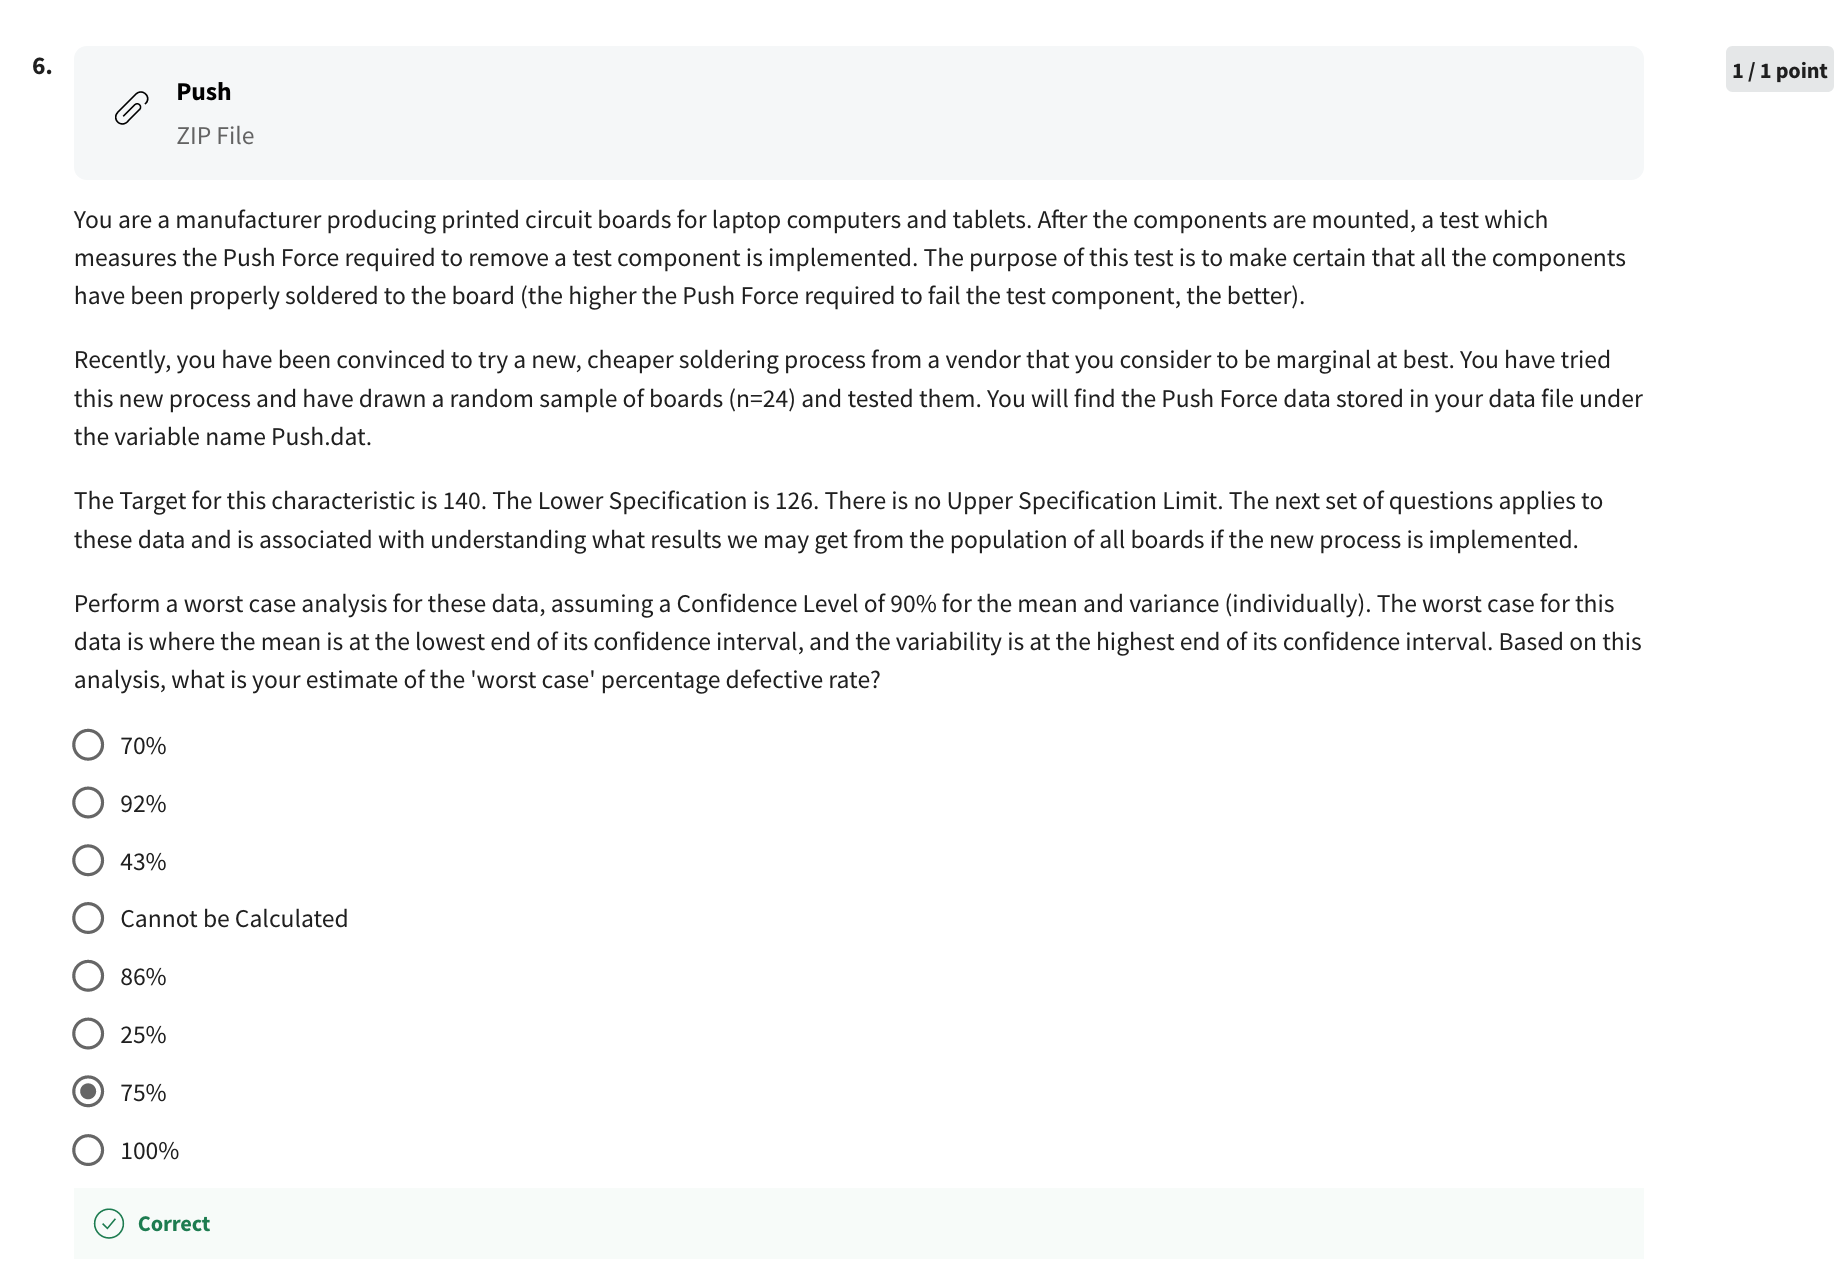
\includegraphics[scale=0.7]{HW6/p8.png}
\end{center}
\end{figure}

\begin{enumerate}
\item (15 pts) Suppose we start the Ford-Fulkerson algorithm  with  $\textbf{A}$ being the source vertex and $\textbf{F}$ being the sink and \textbf{select the path $A ->C ->B -> E -> D ->F$ in the first iteration (Do not chose the first A-F path on your own).} Complete all the iterations of Ford-Fulkerson to find the Max-Flow (including the first round that is incomplete).
Clearly show each round with \\
\begin{enumerate}
\item The path that you are selecting in that round.
\item The bottleneck edge on this path.
\item The additional flow that you push from the source by augmenting (pushing maximum allowed flow along) this selected augmenting path.
\item The residual graph with the residual capacities (on both the forward and backward) edges.
\end{enumerate}
Also, report the Max-Flow after the algorithm terminates.

\makenonemptybox{6in}{}
\clearpage

\item (5 pts) Draw the graph and show the final flow f(e) for the edges of the original graph when the Ford-Fulkerson algorithm terminates.
\makenonemptybox{3in}{}

\item (5 pts) Find the minimum capacity cut with respect to the capacities on the original graph. Is this minimum capacity equal to the Max-Flow that you earlier identified? Justify your answer in a sentence. Also, list the  edges that are part of the min-cut and are saturated (can't carry any more flow).
\makenonemptybox{3in}{}
\end{enumerate}

\item{\itshape \textbf{Extra Credit Question 1 (5 pts)}
    For this extra credit question, please refer the leetcode link provided below or click \href{https://leetcode.com/problems/cheapest-flights-within-k-stops/}{here}. Multiple solutions exist to this question ranging from brute force to the most optimal one. Points will be provided based on Time and Space Complexities relative to that of the most optimal solution.

    Please provide your solution with proper comments which carries points as well.}
    
   \url{https://leetcode.com/problems/cheapest-flights-within-k-stops/}

    % Paste your code in the verbatim tag below
\begin{verbatim}
Replace this text with your source code inside of the .tex document
\end{verbatim}	

\item{\itshape \textbf{Extra Credit Question 2 (5 pts)}
    For this extra credit question, please refer the leetcode link provided below or click \href{https://leetcode.com/problems/pacific-atlantic-water-flow/}{here}. Multiple solutions exist to this question ranging from brute force to the most optimal one. Points will be provided based on Time and Space Complexities relative to that of the most optimal solution.

    Please provide your solution with proper comments which carries points as well.}
    
   \url{https://leetcode.com/problems/pacific-atlantic-water-flow/}

    % Paste your code in the verbatim tag below
\begin{verbatim}
Replace this text with your source code inside of the .tex document
\end{verbatim}	

\end{enumerate}
\end{document}


